\subsubsection{} Генерация криптографических ключей.
\label{sec:eng:performance:rsakeygen}

Метод \texttt{generateRSAKeyPair} необходим для генерации пары \textit{RSA} ключей (публичного и приватного), а метод \texttt{generateAESKey} -- для генераци симметричного \textit{AES} ключа. На рисунке \ref{sec:eng:performance:rsakeygen:code} приведён код для тестирования метода генерации пары \textit{RSA} ключей, а на рисункe \ref{sec:eng:performance:result} -- результаты измерений генерации \textit{RSA} и \textit{AES} ключей соответственно.

\begin{figure}[h]
  \lstinputlisting{inc/src/perf/rsakeygen.swift}
   \caption{Тестовый метод для метода генерации пары RSA ключей}
   \label{sec:eng:performance:rsakeygen:code}
\end{figure}

\begin{figure}[h]
  \centering
    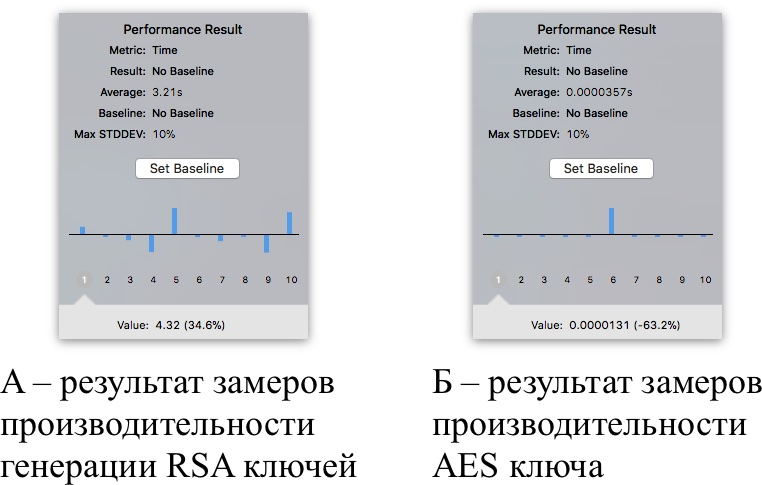
\includegraphics[width=0.75\textwidth]{inc/img/key_generation_performance_test}
  \caption{Результаты тестов производительноси генерации криптографических ключей}
  \label{sec:eng:performance:result}
\end{figure}

\FPeval{\rsaKeyGenMesaureMax}{62.4}
\FPeval{\rsaKeyGenMesaureMin}{11.3}
\FPeval{\rsaKeyGenMesaureAverage}{32.1}
\FPeval{\perfDevRSAKeyGen}{clip(round(((\rsaKeyGenerationMaxValue - (\rsaKeyGenMesaureMax + \rsaKeyGenMesaureMin + \rsaKeyGenMesaureAverage) / 3) / \rsaKeyGenerationMaxValue * 100), 2))}

Рассчитаем отклонение от предельно допустимого значения генерации \textit{RSA} ключа, подставив значения в формулу (\ref{perfDifEquation}):
\begin{center}
\(\perfDev = (\num{\rsaKeyGenerationMaxValue} - \frac{\num{\rsaKeyGenMesaureMax} + \num{\rsaKeyGenMesaureMin} + \num{\rsaKeyGenMesaureAverage}}{\num{3}}) \cdot \frac{\num{1}}{\num{\rsaKeyGenerationMaxValue}} \cdot 100  = \num{\perfDevRSAKeyGen} \, \text{\%}\)
\end{center}

\FPeval{\aesKeyGenMesaureMax}{0.00353}
\FPeval{\aesKeyGenMesaureMin}{0.0000157}
\FPeval{\aesKeyGenMesaureAverage}{0.000357}
\FPeval{\perfDevAESKeyGen}{clip(round(((\aesKeyGenerationMaxValue - (\aesKeyGenMesaureMax + \aesKeyGenMesaureMin + \aesKeyGenMesaureAverage) / 3) / \rsaKeyGenerationMaxValue * 100), 2))}

Аналогичным образом расчитаем отклонение от предельно допустимого значения генерации \textit{AES} ключа:
\begin{center}
\(\perfDev = (\num{\aesKeyGenerationMaxValue} - \frac{\num{\aesKeyGenMesaureMax} + \num{\aesKeyGenMesaureMin} + \num{\aesKeyGenMesaureAverage}}{\num{3}}) \cdot \frac{\num{1}}{\num{\aesKeyGenerationMaxValue}} \cdot 100  = \num{\perfDevAESKeyGen} \, \text{\%}\)
\end{center}